\documentclass{ximera}

\newcommand{\RR}{\mathbb R}
\renewcommand{\d}{\,d}
\newcommand{\dd}[2][]{\frac{d #1}{d #2}}
\renewcommand{\l}{\ell}
\newcommand{\ddx}{\frac{d}{dx}}
\newcommand{\dfn}{\textbf}
\newcommand{\eval}[1]{\bigg[ #1 \bigg]}


\author{Bart Snapp
}
\license{Creative Commons 4.0 By-SA}

\begin{document}
A table of gradient vectors for a function $F:\R^2\to\R$ is
given below:
\begin{image}
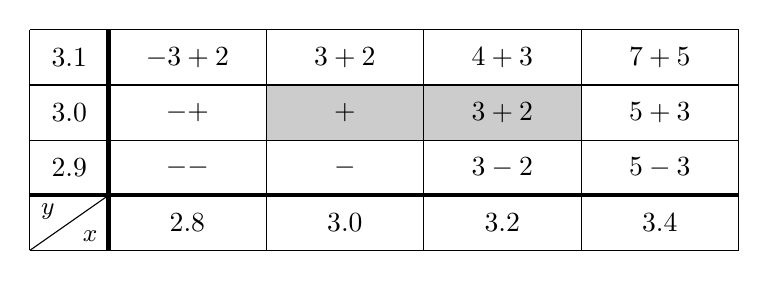
\begin{tikzpicture}[x=1cm,y=.7cm]

  \draw[fill=white!80!black]
  (3,3) -- (7,3) --(7,2) -- (3,2)--cycle;
  
  \draw (0,0) grid [step=1] (1,4);
  \draw (3,4) -- (3,0);
  \draw (5,4) -- (5,0);
  \draw (7,4) -- (7,0);
  \draw (9,4) -- (9,0);
  
  \draw (0,0) -- (9,0);
  \draw (0,1) -- (9,1);
  \draw (0,2) -- (9,2);
  \draw (0,3) -- (9,3);
  \draw (0,4) -- (9,4);


  
  \draw[ultra thick] (0,1)--(9,1);
  \draw[ultra thick] (1,4)--(1,0);
  
  \draw (0,0) -- (1,1);
  %\node at (.9,.9) [below left,inner sep=1pt] {\small$y$};
  %\node at (0.1,.1) [above right,inner sep=1pt] {\small$x$};
  \node at (.1,.9) [below right,inner sep=1pt] {\small$y$};
  \node at (0.9,.1) [above left,inner sep=1pt] {\small$x$};
  
  
  %% x-values
  \node at (2,.5) {$2.8$};
  \node at (4,.5) {$3.0$};
  \node at (6,.5) {$3.2$};
  \node at (8,.5) {$3.4$};
  
  %% y-values
  \node at (0.5,1.5) {$2.9$};
  \node at (0.5,2.5) {$3.0$};
  \node at (0.5,3.5) {$3.1$};
  
  
  %% vectors
  %% top row
  \node at (2,3.5) {$-3\veci+2\vecj$};
  \node at (4,3.5) {$3\veci+2\vecj$};
  \node at (6,3.5) {$4\veci+3\vecj$};
  \node at (8,3.5) {$7\veci+5\vecj$};

  %% second row
  \node at (2,2.5) {$-\veci+\vecj$};
  \node at (4,2.5) {$\veci+\vecj$};
  \node at (6,2.5) {$3\veci+2\vecj$};
  \node at (8,2.5) {$5\veci+3\vecj$};
  
  %% bottom row
  \node at (2,1.5) {$-\veci-\vecj$};
  \node at (4,1.5) {$\veci-\vecj$};
  \node at (6,1.5) {$3\veci-2\vecj$};
  \node at (8,1.5) {$5\veci-3\vecj$};
  
\end{tikzpicture}
\end{image}
\begin{exercise}
  Find $\grad F(3.4,2.9)$.

\end{exercise}

\begin{exercise}
  Suppose that $\vec{p}(t)= \vector{5t-11.8,4t-9.1}$. Compute
  $\dd{t}F(\vec{p}(t))$ evaluated at $t=3$.
\end{exercise}

\begin{exercise}
  Give your best guess for the $(x,y)$-coordinates that give local
  extrema. \textbf{Identify this extrema as a local maximum or minimum.}
\end{exercise}

\begin{exercise}
  Give a formula for a line passing through the point $(2.8, 3.1)$
  such that when $F$ is constrained to your line, $F$ has an extrema
  at the point $(2.8, 3.1)$.

\end{exercise}

\begin{exercise}
  Let $R$ be the shaded region above, and assume our gradient vectors
  are sampled in some reasonable way.  \textbf{Estimate} the surface
  area of $F$ over $R$ as we did in class and in the text.  As a
  gesture of friendship, we remind you that $S = \iint_R \sqrt{1+
    \pp[F]{x}^2 + \pp[F]{y}^2} \d A$. You do \textbf{not} need to
  simplify.
\end{exercise}
\end{document}
